\documentclass[11pt]{article}
\usepackage[a4paper,margin=2cm]{geometry}
\title{%
    The Hare and the Tortoise \\
    \large A Mini Project \\
}
\author{Patrick Pellacani Muller}
\setcounter{section}{-1}

\usepackage{float}
\usepackage{siunitx}
\usepackage{minted}
\usemintedstyle{colorful}

% tikz setup
\usepackage{tikz}
\usetikzlibrary{positioning,shapes.geometric,arrows.meta}

\tikzstyle{startstop} = [rectangle, rounded corners, minimum width=3cm, minimum height=0.8cm, text centered, draw=black, fill=gray!20, font=\small]
\tikzstyle{process} = [rectangle, minimum width=3cm, minimum height=0.8cm, text centered, draw=black, fill=gray!10, font=\small]
\tikzstyle{decision} = [diamond, aspect=2, text centered, draw=black, fill=gray!10, font=\small, inner sep=3pt]
\tikzstyle{io} = [trapezium, trapezium left angle=70, trapezium right angle=110,
                   minimum width=3cm, minimum height=0.8cm, text centered, draw=black, fill=gray!10, font=\small]
\tikzstyle{subprog} = [
    rectangle, minimum width=3cm, minimum height=0.8cm,
    text centered, draw=black, fill=gray!5, font=\small,
    inner xsep=8pt,
    path picture={
        \draw[line width=0.8pt]
            ([xshift=0.15cm]path picture bounding box.north west) --
            ([xshift=0.15cm]path picture bounding box.south west);
        \draw[line width=0.8pt]
            ([xshift=-0.15cm]path picture bounding box.north east) --
            ([xshift=-0.15cm]path picture bounding box.south east);
    }
]
\tikzstyle{arrow} = [thick, ->, >=Stealth]
\tikzstyle{structnode} = [
    rectangle,                 % Shape
    draw=black,                % Border color
    thick,                     % Slightly thicker border
    rounded corners=2pt,       % Optional: slightly rounded
    minimum width=2cm,       % Width
    minimum height=1cm,        % Height
	inner xsep=5pt,
    text centered,             % Centered text
    fill=gray!15,              % Subtle background
    font=\small                % Font size
]



\usepackage{datetime}
\newdate{writing_date}{13}{10}{2025}
\date{\displaydate{writing_date}}

\usepackage{biblatex}
\addbibresource{sources.bib}

\begin{document}


\maketitle


\tableofcontents


\section{Introduction}
\subsection{Purpose}
The main purpose of the program is entertainment as it is a game to be enjoyed. It
simulates the classic story of the tortoise and the hare. To make the game enjoyable,
the user is asked to bet on either the hare or the tortoise. This money is then used
to play another round as long as the user has enough money. The aim for the user is to
play as many rounds as possible.
\subsection{Intended user}
Possible users of the program are younger children as the game loop is very simple and
may not appeal as much to older children, teenagers or adults. It should therefore be easy
to use and understand. However, there may be moral considerations when aiming a game that
involves gambling and betting to (young) children. This is combated by using the artificial
currency of "carrots" which the user can use to bet on an animal. If they win, they gain
"carrots". The aim of the game is therefore not to make the most money gambling but instead
to collect the most "carrots" in a given number of rounds to feed \cite{hare-diet,tortoise-diet}
the animals. The animals require feeding to play another round.
\subsection{Functionality}
A simple pseudo-random number generator based simulation of the game of ``the hare and the
tortoise''. The initial parameters - which are open for change and improvement -
for the simulation are:
\begin{itemize}
	\item The game is divided into rounds, and finishes when the first person reaches
	      \qty{1000}{\metre}
	\item Each round the tortoise moves \qtyrange{5}{10}{\metre}
	\item Each round the hare moves \qtyrange{8}{15}{\metre}
	\item However, there is a \qty{25}{\percent} chance that the hare doesn't move
\end{itemize}

The betting system has odds set out to increase the user's "carrots" slightly if the fee for
playing a new round is not taken into account. However, as there is a fee to play each round,
on average, the number of carrots that a player has tends to zero.

\subsection{Why a computational approach was used}
\label{sec:approach}
A computational approach is best here as the races can be quite long and can be simulated more
quickly. As the game is aimed at children, a lengthy process of e.g. rolling dice may be unrealistic
as most children will be bored before the first game even finishes. For example, on average the
tortoise would take \(\frac{1000}{7.5} \approx 134\) rounds to complete a race. Assuming a dice roll
every \qty{2}{\second}, this will take
\(134 \times \qty{2}{\second} = \qty{268}{\second} \approx \qty{4.5}{\minute}\) of dice rolls.
Furthermore, betting and keeping track of carrots can also be tedious and is therefore managed by
a computer.

The programming language that is used in this project is Rust \cite{rust} which provides a
safe, compiled language. The main reasons for this is to offer security and help with data
validation. As the language is precompiled into machine code, the user doesn't have to install
an interpreter like Python or the JRE. This may reduce the complexity of the install process
for the users, which is beneficial as the game is aimed at young children. Given that most
desktop PCs and laptops run either Windows 10/11 x86\_64/arm64 or macOS arm64 \cite{os},
and Rust can cross-compile for all of those CPU architectures and operating systems, compatability
problems shouldn't cause a major issue. By using a compiled language, the program will run
more efficiently, which isn't a major concern right now but allows for a better integration of a
more complex UI and game mechanics later. Furthermore, the game is aimed at children who often do
not have the money to buy powerful PCs, and performance could be a major factor later if new
features get added. From a development point of view, using Rust allows for the use of modern tools
such as functional programming to keep code neat, tidy, legible and extensible. The strict typing rules
and borrow checker ensures memory safety and reduces logic and security errors.

\section{Data structures}
The constants used in the program are defined in Table~\ref{tab:consts}. These are carefully chosen
to allow for quick changes of the game's main parameters. Variables are listed in Table~\ref{tab:vars}.
Great care has been taken to reduce unnecessary variables while keeping code clean and readable, as
well as ready for future expansion. Therefore, four custom structs (structured groups of data) as well as two
enums (list of structs sharing similar properties) are used for modularity, and their relationship as well as
structure can be seen in Figure~\ref{fig:structs}.

The decision to make \texttt{Animal} an enum has the upside of allowing the addition of  more animals
while minimizing the risk that the new animals aren't properly implemented in code as Rust ensures that
all enum elements are covered whenever one is using enums. This improves the program's extensibility
and safety greatly.

\texttt{RoundResult} being an enum allows for the use of match ... case syntax to keep code clean, and makes
testing easier as all possible varations are covered more easily.

The four structs used allow the code to stay segmented and modular, therefore allowing a team of developers
to work on the project simutaneously. For instance, when winning is being implemented, one doesn't have
to think about how the betting mechanic works, and instead leave that up to the \texttt{Bet} struct
to hanlde. This improves efficiency when developing and allows for greater extensibility later in the
program's lifecycle.

\begin{table}[!h]
	\centering
	\begin{tabular}{ | c c | }
		\hline
		Name                               & Type                \\
		\hline
		\texttt{RACE\_LENGTH}              & \texttt{f64}        \\
		\texttt{TORTOISE\_SPEED\_INTERVAL} & \texttt{(f64, f64)} \\
		\texttt{HARE\_SPEED\_INTERVAL}     & \texttt{(f64, f64)} \\
		\texttt{HARE\_SLEEP\_CHANCE}       & \texttt{f64}        \\
		\texttt{FIXED\_COSTS}              & \texttt{i32}        \\
		\texttt{INITIAL\_BALANCE}          & \texttt{i32}        \\
		\hline
	\end{tabular}
	\caption{Constants used in the game}%
	\label{tab:consts}
\end{table}
\begin{table}[!h]
	\centering
	\begin{tabular}{ | c c | }
		\hline
		Name              & Type                     \\ \hline
		\texttt{winners}  & \texttt{mut WinnerTable} \\
		\texttt{balance}  & \texttt{mut i32}         \\
		\texttt{bet}      & \texttt{mut Bet}         \\
		\texttt{animals}  & \texttt{mut Vec<Animal>} \\ \hline
		\texttt{tortoise} & \texttt{Tortoise}        \\
		\texttt{result}   & \texttt{Result}          \\
		\texttt{hare}     & \texttt{Hare}            \\ \hline
	\end{tabular}
	\caption{Variables used in the game loop}
	\label{tab:vars}
\end{table}

\begin{figure}[!h]
	\centering
	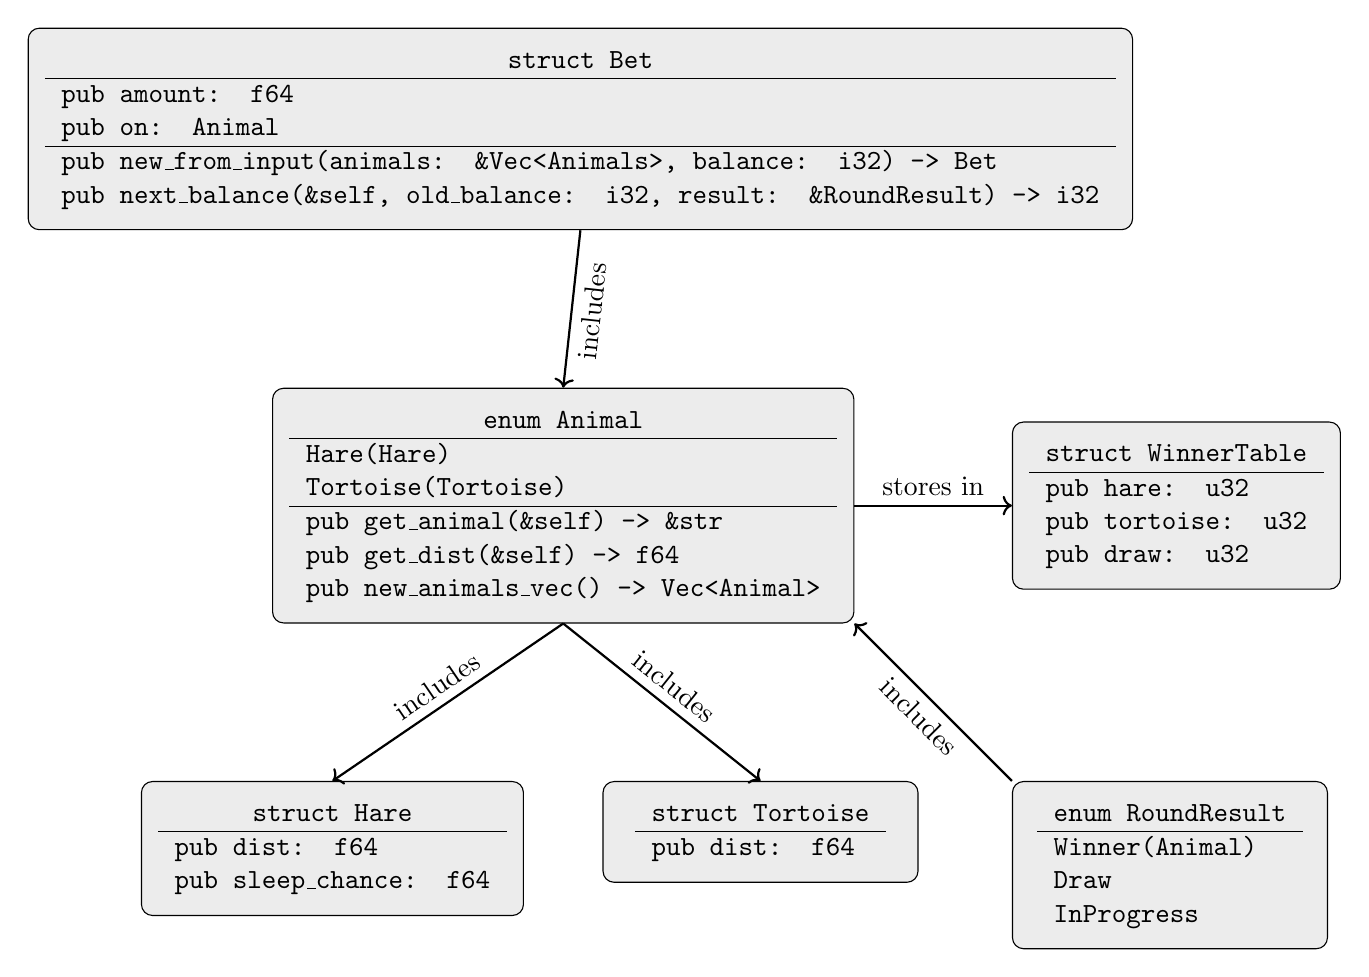
\begin{tikzpicture}[
			struct/.style={
					rectangle,
					draw=black,
					rounded corners,
					fill=gray!15,
					minimum width=4cm,
					inner sep=6pt,
					font=\ttfamily,
				}
		]

		% Animal enum
		\node[struct] (animal) {
			\begin{tabular}{l}
				\multicolumn{1}{c}{enum Animal}        \\ \hline
				Hare(Hare)                             \\
				Tortoise(Tortoise)                     \\ \hline
				pub get\_animal(\&self) -> \&str       \\
				pub get\_dist(\&self) -> f64           \\
				pub new\_animals\_vec() -> Vec<Animal> \\
			\end{tabular}
		};

		% Hare struct
		\node[struct, below left=2.0cm and -3.2cm of animal] (hare) {
			\begin{tabular}{l}
				\multicolumn{1}{c}{struct Hare} \\ \hline
				pub dist: f64                   \\
				pub sleep\_chance: f64          \\
			\end{tabular}
		};

		% Tortoise struct
		\node[struct, below right=2.0cm and -3.2cm of animal] (tortoise) {
			\begin{tabular}{l}
				\multicolumn{1}{c}{struct Tortoise} \\ \hline
				pub dist: f64                       \\
			\end{tabular}
		};

		% WinnerTable struct
		\node[struct, right=2cm of animal] (winner) {
			\begin{tabular}{l}
				\multicolumn{1}{c}{struct WinnerTable} \\ \hline
				pub hare: u32                          \\
				pub tortoise: u32                      \\
				pub draw: u32                          \\
			\end{tabular}
		};

		% Bet struct
		\node[struct, above right=2cm and -10.5cm of animal] (bet) {
			\begin{tabular}{l}
				\multicolumn{1}{c}{struct Bet}                                             \\ \hline
				pub amount: f64                                                            \\
				pub on: Animal                                                             \\ \hline
				pub new\_from\_input(animals: \&Vec<Animals>, balance: i32) -> Bet         \\
				pub next\_balance(\&self, old\_balance: i32, result: \&RoundResult) -> i32 \\
			\end{tabular}
		};

		% RoundResult struct
		\node[struct, below right=2cm and 2cm of animal] (roundresult) {
			\begin{tabular}{l}
				\multicolumn{1}{c}{enum RoundResult} \\ \hline
				Winner(Animal)                       \\
				Draw                                 \\
				InProgress                           \\
			\end{tabular}
		};

		% Connections
		\draw[->, thick] (animal.east) -- node[above,sloped]{stores in} (winner.west);
		\draw[<-, thick] (hare.north) -- node[above,sloped]{includes} (animal.south);
		\draw[<-, thick] (tortoise.north) -- node[above,sloped]{includes} (animal.south);
		\draw[->, thick] (bet.south) -- node[below,sloped]{includes} (animal.north);
		\draw[->, thick] (roundresult.north west) -- node[below,sloped]{includes} (animal.south east);
	\end{tikzpicture}
	\caption{The structure diagram of the \texttt{struct}s \texttt{Hare}, \texttt{Tortiose}}
	\label{fig:structs}
\end{figure}

\section{Outline of Program}
\subsection{Overview of main algorithm}
The flowchart in Figure~\ref{fig:flw-prgm} outlines clearly the main program loop and how the main
part of the program calls the smaller modules. Below, the same idea can be found, written in pseudocode
(See Listing~\ref{lst:psd-overview}). It is is meant as a visual and textual overview for later
reference, respectively.

The game loop consists of two main parts: simulating a race, and taking and evaluating bets. These aim to
give an engaging yet simple game loop which can be easily understood by younger users but still be
enjoyable. Savegame functionality is also implemented.

\begin{listing}
	\begin{minted}[frame=lines, linenos, autogobble]{text}
	DEF balance
	load_savegame()
	DO
		VAR bet = bet_from_input()
		DO
			VAR result = play_and_get_result()
			IF result.ended() THEN
			BREAK
			ENDIF
		WHILE
		announce_winner()
		store_winner()
		update_balance()
		IF balance < 0 THEN
			break
		ENDIF
	WHILE Input("Another Race?")
	output_stats()
	write_savegame()
        \end{minted}
	\caption{A pseudocode overview of the main program.}
	\label{lst:psd-overview}
\end{listing}
\begin{figure}[!h]
	\centering
	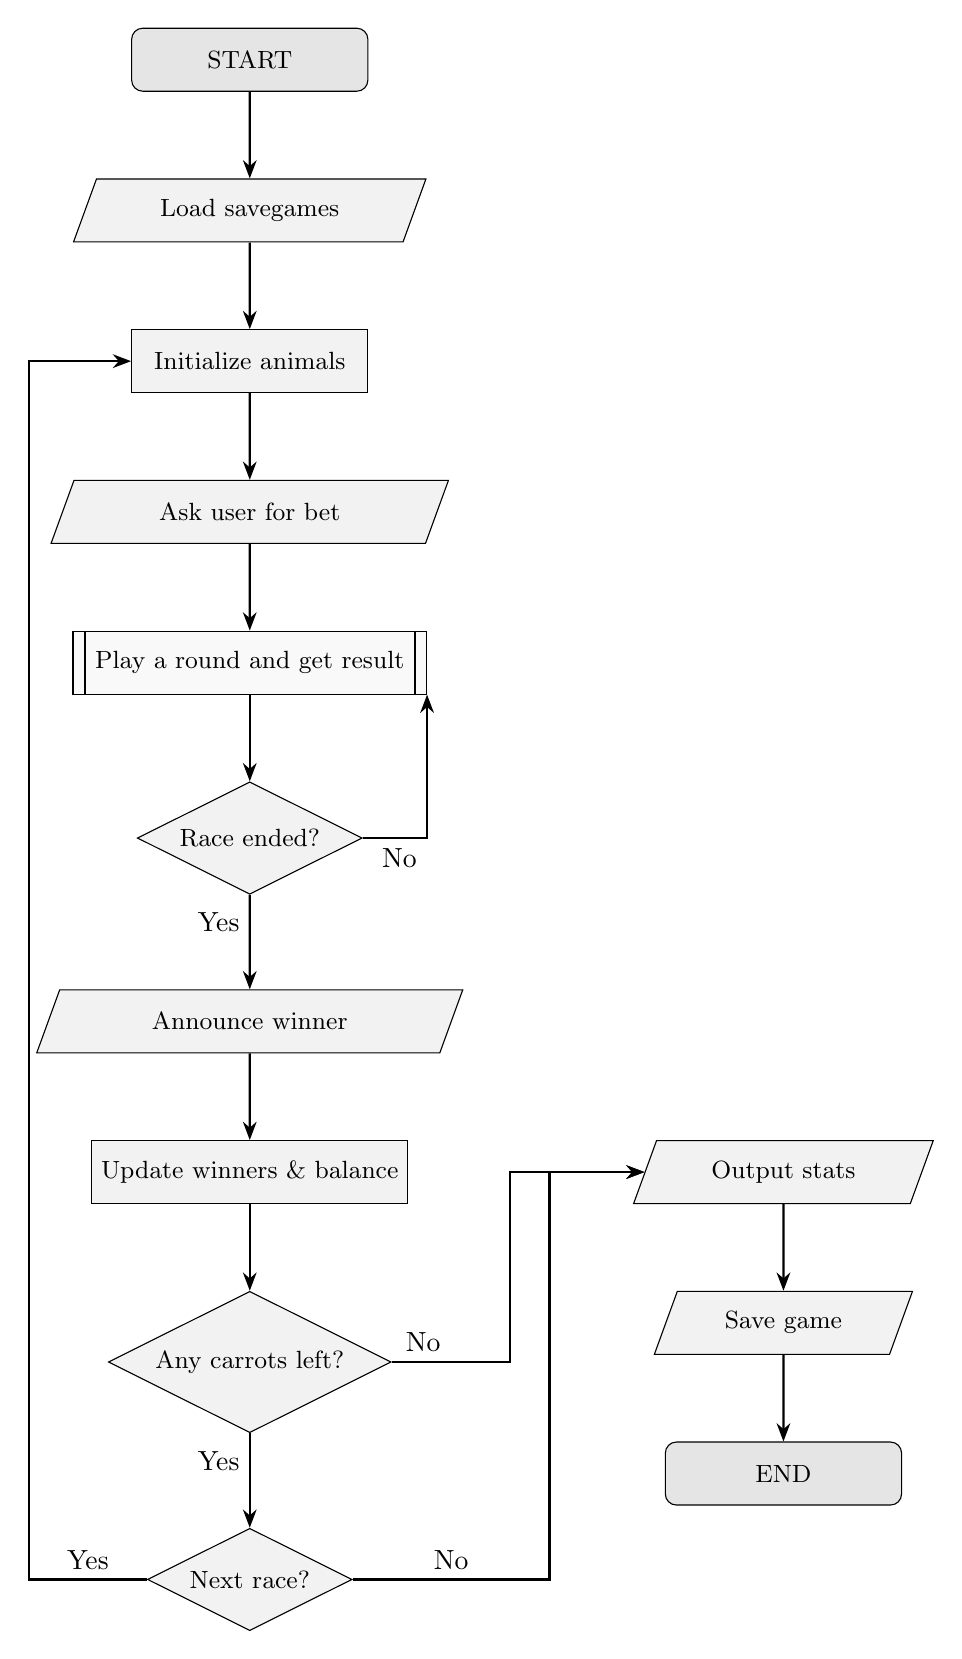
\begin{tikzpicture}[node distance=1.1cm]

		% Nodes
		\node (start) [startstop] {START};

		\node (load_sg) [io, below=of start] {Load savegames};

		\node (init_anims) [process, below=of load_sg] {Initialize animals};
		\node (init_bet) [io, below=of init_anims] {Ask user for bet};

		\node (res) [subprog, below=of init_bet] {Play a round and get result};
		\node (racecheck) [decision, below=of res] {Race ended?};

		\node (announce) [io, below=of racecheck, yshift=-0.1cm] {Announce winner};
		\node (store) [process, below=of announce] {Update winners \& balance};

		\node (moneycheck) [decision, below=of store] {Any carrots left?};

		\node (againcheck) [decision, below=of moneycheck, yshift=-0.1cm] {Next race?};


		\node (stats) [io, right=3cm of store] {Output stats};
		\node (write_sg) [io, below=of stats] {Save game};
		\node (stop) [startstop, below=of write_sg] {END};

		% Arrows
		\draw [arrow] (start) -- (load_sg);
		\draw [arrow] (load_sg) -- (init_anims);
		\draw [arrow] (init_anims) -- (init_bet);
		\draw [arrow] (init_bet) -- (res);
		\draw [arrow] (res) -- (racecheck);

		\draw [arrow] (racecheck.east) -| node[anchor=north east] {No} (res.south east);
		\draw [arrow] (racecheck) -- node[anchor=south east] {Yes} (announce);

		\draw [arrow] (announce) -- (store);
		\draw [arrow] (store) -- (moneycheck);

		\draw [arrow] (moneycheck.south) -- node[anchor=south east] {Yes} (againcheck.north);
		\draw [arrow] (moneycheck.east) -- node[anchor=south east] {No} ++(+1.5,0) |- (stats);

		\draw [arrow] (againcheck.west) -- node[anchor=south] {Yes} ++(-1.5,0) |- (init_anims);
		\draw [arrow] (againcheck.east) -- node[anchor=south] {No} ++(+2.5,0) |- (stats);


		\draw [arrow] (stats) -- (write_sg);
		\draw [arrow] (write_sg) -- (stop);
	\end{tikzpicture}
	\caption{Flowchart of the main program}
	\label{fig:flw-prgm}
\end{figure}
\subsection{Modularity}
\label{sec:modules}

This project is split into two parts: a binary crate and a library crate. Crates are a collection of code
in Rust which are equivalent to libraries in other build systems. The advantage of splitting the main binary
(which contains any code specific to this version of the program) and a library crate (which can be reused
across multiple projects) is greater flexibility when updating the program.

The four modules in the library crate will be \texttt{io}, \texttt{race}, \texttt{betting} and \texttt{stats}.
These can be independently developed, tested, debugged and refined. A visual overview of modules can be found
in Figure~\ref{fig:structure}. Below is an explanation of each of the modules (and respective submodules
found in the crate) and their function:
\begin{itemize}
	\item I/O (stands for Input/Output): manages displaying results to the user, getting input
	      from the user, including any validation necessary; furthermore, \texttt{io} crate also manages
	      savegames and stats management, as all these are part of inputting and outputting data for the user;
	      contains two submodules: \texttt{cli} and \texttt{savegames}. Possibility for future GUI interfaces
	      would be implemented in this crate using a \texttt{gui} submodule.
	\item Race: manages the race logic, including movement of the hare and tortoise, and the end
	      condition; contains two \texttt{mod}s: \texttt{movement} and \texttt{finish}
	\item Betting: manages the betting mechanic, including odds, saving money and the price to pay per round;
	      it contains the \texttt{Bet} struct which allows for this functionality.
	\item Stats: manages keeping race statistics like which animal won and any ties that happened; contains
	      the \texttt{WinnerTable} struct to accopmplish this
\end{itemize}

The binary crate is the final program that the user runs. It links the individual elements together as
showin in Figure~\ref{fig:flw-prgm}. The pseudocode for this crate can be found in
Listing~\ref{lst:psd-overview}. Separating the binary crates from the libraries allows for simple
such as changing the order of the game loop, or compiling different games with different game loops by
reusing the existing library crates and building a new binary crate. This would allow for different versions of
the same game, for example differing in interface or difficulty, to be compiled from a single library.

\begin{figure}[!h]
	\centering
	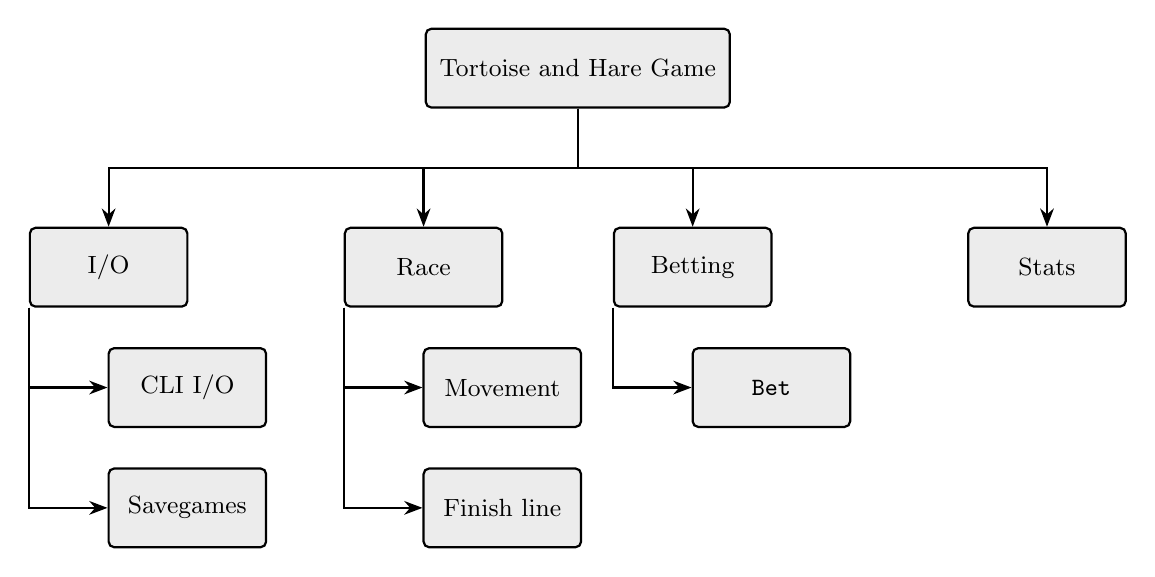
\begin{tikzpicture}[node distance=0.5cm]

		% Top-level module
		\node[structnode] (game) {Tortoise and Hare Game};

		% Input module
		\node[structnode, below left=1.5cm and 3cm of game] (io) {I/O};
		\node[structnode, below=of io, xshift=1cm] (cli_io) {CLI I/O};
		\node[structnode, below=of cli_io] (storage) {Savegames};


		% Race module
		\node[structnode, below left=1.5cm and -1.0cm of game] (race) {Race};
		\node[structnode, below=of race, xshift=1cm] (move) {Movement};
		\node[structnode, below=of move] (end) {Finish line};

		% Betting module
		\node[structnode, below right=1.5cm and -1.5cm of game] (bet) {Betting};
		\node[structnode, below=of bet, xshift=1cm] (betstruct) {\texttt{Bet}};

		% Stats module
		\node[structnode, below right=1.5cm and 3cm of game] (stats) {Stats};

		% Arrows
		\draw[arrow] (game.south) -- ++(0,-0.75) -| (io);
		\draw[arrow] (io.south west) |- (cli_io);
		\draw[arrow] (io.south west) |- (storage);

		\draw[arrow] (game.south) -- ++(0,-0.75) -| (race);
		\draw[arrow] (race.south west) |- (move);
		\draw[arrow] (race.south west) |- (end);

		\draw[arrow] (game.south) -- ++(0,-0.75) -| (bet);
		\draw[arrow] (bet.south west) |- (betstruct);

		\draw[arrow] (game.south) -- ++(0,-0.75) -| (stats);
	\end{tikzpicture}
	\caption{Structure diagram outlining the three library crates and their functions}
	\label{fig:structure}
\end{figure}

\section{In-depth Gameplay analysis}
During gameplay testing, a large problem that occured is that the hare nearly always wins. The
probabilities are not chosen well enough to allow for a balanced gameplay experience. Due to this,
ties are also nearly never happen.

A starting carrots of 300 and a round-on-round cost of 20 carrots were chosen as they seem to deliver
balanced gameplay which is fun but still leads to the eventual end of the game.

The gameplay is relatively engaging for about 5 minutes, after which it becomes boring. This may be the result of the game being
entirely CLI based, and therefore a good extension to the game would be adding a GUI.

As draws should be possible, gameplay testing has shown that the only way they realistically happen is to disregard any progress
past the finishing distance. This means that if the hare's distance is 1000.1m and the tortoise's distance is 1008.3m after a
given round, that is counted as a draw. The user doesn't know this and it therefore positively impacts gameplay as it adds to the
excitement by making draws possible, even though this may be slightly unrealistic.

\section{Testing}
\subsection{Inputs and testing approach}
The main data inputs are:
\begin{itemize}
	\item Choosing between betting on the tortoise or hare
	\item Entering the amount of money to bet
	\item Deciding whether or not to play another round
\end{itemize}

Because Rust is used as the programming language (see Section~\ref{sec:approach}), data safety
and errors such as buffer overflow errors are dealt with by the language. However, testing that
these safeguards are in place properly is still good practice, especially as the default response
to such an error in Rust would be a ``\texttt{panic}'', which stops the program abruptly and may
cause users to be annoyed at the program if they experience such an error in the middle of the game.
Furthermore, these errors are not supposed to happen in production and are a safety mechanism rather
than a feature to rely on.

To ensure the correct functionality of individual crates and modules, unit testing will be used throughout
the development phase. This ensures that the individual crates and modules outlined in Section~\ref{sec:modules}
are working as intended, by testing them independently from other parts of the program. The approach that is
used for unit testing is outlined in Section ~\ref{sec:unit-test}

Furthermore, testing after development with valid, boundary, invalid and erroneous data will ensure
that the whole program works as expected. This data is outlined in Section~\ref{sec:whole-test}.
\subsection{Unit Testing}
\label{sec:unit-test}
Unit testing was sucessfully used during the development process in the \texttt{race}, \texttt{betting} and \texttt{stats}
modules. This can be exemplified when unit testing was used to catch a logic error in the \texttt{betting} module which
didn't account for draws properly.

The testing framework used is the default built-in testing framework part of the Rust language, which can be run using
\texttt{cargo test}, resulting in the output seen in Listing~\ref{lst:test-fail} when a unit test failed as the draw logic was
programmed wrong.

Test data used for \texttt{betting} unit tests can be found in Table~\ref{tab:unit-tests-betting}.
Table~\ref{tab:unit-tests-stats} contains \texttt{stats} unit tests. This unit test starts with an empty \texttt{WinnerTable}
struct and populates it as shown in the Table~\ref{tab:unit-tests-stats}. Finally, the \texttt{race} module is tested in two
parts. The movement submodule is tested by first giving the hare a \texttt{sleep\_chance} of 1.0 and ensuring it doesn't move.
Then, the pseudo-random number generator is seeded with a special seed, whose outcome is known at compile time, and can therefore
be predicted. This is used to test the random sleep chance with multiple known values.
Finally, both the tortoise and a hare with a sleep chance of 0.0 are moved multiple times and it is ensured that they each time
their movement is within their respective movement interval. The test data used for testing the \texttt{finish} submodule is
shown in Table~\ref{tab:unit-tests-finish}.



\begin{table}[!h]
	\centering
	\begin{tabular}{ | c c c c | c | c | }
		\hline
		Round state  & Bal. before & Bet on   & Bet amount & Exp. bal. after & Act bal. after \\ \hline
		Hare won     & 100         & Hare     & 10         & 90              & 90             \\
		Hare won     & 100         & Tortoise & 10         & 70              & 70             \\
		Tortoise won & 200         & Hare     & 50         & 130             & 130            \\
		Tortoise won & 200         & Tortoise & 50         & 230             & 230            \\
		Draw         & 500         & Tortoise & 200        & 280             & 280            \\
		Draw         & 500         & Hare     & 200        & 280             & 280            \\
		In Progress  & 200         & Tortoise & 50         & 200             & 200            \\
		In Progress  & 1000        & Hare     & 350        & 1000            & 1000           \\ \hline
	\end{tabular}
	\caption{\texttt{betting} unit test data}
	\label{tab:unit-tests-betting}
\end{table}

\begin{table}[!h]
	\centering
	\begin{tabular}{ | c | c c c | c c c |}
		\hline
		Result       & Exp. hare & Exp. tortoise & Exp. draw & Act. hare & Act. tortoise & Act. draw \\ \hline
		Draw         & 0         & 0             & 1         & 0         & 0             & 1         \\
		In Progress  & 0         & 0             & 1         & 0         & 0             & 1         \\
		Hare won     & 1         & 0             & 1         & 1         & 0             & 1         \\
		Tortoise won & 1         & 1             & 1         & 1         & 1             & 1         \\
		Tortoise won & 1         & 2             & 1         & 1         & 2             & 1         \\ \hline
	\end{tabular}
	\caption{\texttt{stats} unit test data}
	\label{tab:unit-tests-stats}
\end{table}

\begin{table}[!h]
	\centering
	\begin{tabular}{ | c c | c | c | }
		\hline
		Hare dist & Tortoise dist & Exp. round state & Act. round state \\ \hline
		0         & 0             & In Progress      & In Progress      \\
		0         & 1.7           & In Progress      & In Progress      \\
		2.3       & 1.7           & In Progress      & In Progress      \\
		0         & 1000          & Tortoise won     & Tortoise won     \\
		2.3       & 1003.6        & Tortoise won     & Tortoise won     \\
		1000      & 1000          & Draw             & Draw             \\
		1003.6    & 1000          & Draw             & Draw             \\
		1003.6    & 1003.6        & Draw             & Draw             \\
		1000      & 1003.6        & Draw             & Draw             \\
		1000      & 1.7           & Hare won         & Hare won         \\ \hline
	\end{tabular}
	\caption{\texttt{finish} unit test data}
	\label{tab:unit-tests-finish}
\end{table}

\begin{listing}[!h]
	\begin{minted}[frame=lines]{text}
running 4 tests
test race::movement::tests::test_move_animals ... ok
test betting::tests::test_update_balance ... FAILED
test race::finish::tests::test_winner ... ok
test stats::tests::test_winner_table_update ... ok

failures:

---- betting::tests::test_update_balance stdout ----
You have won your bet and get 10 more carrots.
The animals are hungry need to eat. You give them 20 carrots.
You have lost your bet and have to give 10 carrots away.
The animals are hungry need to eat. You give them 20 carrots.
You have lost your bet and have to give 50 carrots away.
The animals are hungry need to eat. You give them 20 carrots.
You have won your bet and get 50 more carrots.
The animals are hungry need to eat. You give them 20 carrots.

thread 'betting::tests::test_update_balance' panicked at src/betting.rs:113:9:
assertion `left == right` failed
  left: 500
 right: 280
	\end{minted}
	\caption{\texttt{cargo test} output showing some unit tests failing}
	\label{lst:test-fail}
\end{listing}

\subsection{Validation Testing}
\label{sec:whole-test}

Most of the validation testing was done through play testing after the program has finished. This also included testing the
\texttt{io} module, as that is difficult to do using unit tests. The savegame functionality works perfectly, and so does playing
the rounds. To facilitate this testing, different variables were printed to the console one at a time, and manually checked to
make sure that they are behaving as expected. These included \texttt{winners}, \texttt{bet} and \texttt{animals}.

A logic error was cought this way, as at the end of a race the animals were not reset back to 0, and instead carried on racing
from their previous distance. This bug was fixed by resetting the \texttt{animals} vec with a fresh one at the end of every race.

\section{Evaluation}
This game's main shortfalls are the lack of a GUI which makes it less engaging. Furthermore the probablities and money values
would have to be further tweaked to make it a fun to play and balanced. This would include a lot of play testing.
The modular design that this project was built of makes expanding the code to fit new requirements quick and easy.

Another feature that is missing is the ability to save multiple savegames and name the animals however the player wants to. All
of these can be implemented relatively easily by editing the right module.

The testing strategy was a success and cought a few bugs, making the program less frustrating to use for the user and better at
fulfilling its purpose, entertaining the user.


\appendix


\section{Source code}
\begin{samepage}
	The source code is organised as such:
	\begin{minted}{text}
src
|-- betting.rs
|-- io
|   |-- cli.rs
|   `-- savegames.rs
|-- io.rs
|-- lib.rs
|-- main.rs
|-- race
|   |-- finish.rs
|   `-- movement.rs
|-- race.rs
|-- stats.rs
\end{minted}
\end{samepage}

Full source code:
\inputminted[frame=lines]{rust}{../combined.txt}

\printbibliography[heading=bibnumbered]

\end{document}
